\documentclass[12pt,a4paper]{article}
\usepackage[T2A]{fontenc}
\usepackage[utf8]{inputenc}
\usepackage[russian]{babel}
\usepackage{amsmath,amssymb,mathtools}
\usepackage{graphicx,booktabs,array}
\usepackage[section]{placeins}
\usepackage[left=25mm,right=15mm,top=20mm,bottom=20mm]{geometry}
\usepackage{microtype}
\usepackage[unicode,hidelinks]{hyperref}
\usepackage{enumitem}
\setlist{nosep,leftmargin=*}
\setlength{\parindent}{1.25cm}
\setlength{\parskip}{2pt}
\setlength{\textfloatsep}{10pt}
\setlength{\intextsep}{10pt}
\renewcommand{\arraystretch}{1.15}
\newcommand{\dd}{\,\mathrm{d}}
\newcommand{\norm}[1]{\left\lVert#1\right\rVert}
\newcommand{\ip}[2]{\left\langle#1,#2\right\rangle}
\DeclareMathOperator{\Rea}{Re}
\begin{document}
\begin{titlepage}
\begin{center}
\small МИНИСТЕРСТВО НАУКИ И ВЫСШЕГО ОБРАЗОВАНИЯ\\
РОССИЙСКОЙ ФЕДЕРАЦИИ\par
\vspace{5mm}
Федеральное государственное автономное образовательное учреждение\\
высшего образования\\
«Национальный исследовательский Нижегородский\\
государственный университет им. Н. И. Лобачевского»\par
\vspace{5mm}
Институт информационных технологий, математики и механики\par
Направление подготовки: «Прикладная математика и информатика»
\vfill
{\large Отчёт по лабораторной работе № 4\\[4mm]
по уравнениям математической физики\\[5mm]
Тема: «Специальные функции»}
\end{center}
\vspace{15mm}
\begin{flushright}
Выполнили: студенты группы 3823Б1ПМоп2\\
Золкин Иван Александрович\\
Носов Владимир Михайлович\\[5mm]
Проверил: к.\,ф.-м.\,н., доцент\\
Муняев Вячеслав Олегович
\end{flushright}
\vfill
\begin{center}Нижний Новгород\\2026\end{center}
\end{titlepage}

\tableofcontents
\clearpage
\section{Функции Бесселя}
\subsection{Фундаментальная система решений}
Рассмотрим уравнение Бесселя порядка $\nu$:
\begin{equation}\label{eq:bessel}
y''+\frac1x y'+\left(1-\frac{\nu^2}{x^2}\right)y=0,\qquad x>0.
\end{equation}
Подстановка $y=x^s\sum_{k=0}^{\infty}a_kx^{2k}$ даёт
\[
s^2=\nu^2,\qquad
 a_k=-\frac{a_{k-1}}{(s+2k)^2-\nu^2}.
\]
При $s=\nu$ и стандартной нормировке получаем
\begin{equation}\label{eq:Jseries}
J_\nu(x)=\sum_{k=0}^{\infty}
\frac{(-1)^k(x/2)^{2k+\nu}}{k!\,\Gamma(k+\nu+1)}.
\end{equation}
Для $\nu\notin\mathbb Z$ решения $J_\nu$ и $J_{-\nu}$ независимы. Удобная фундаментальная система, пригодная также при целых порядках, имеет вид
\[
J_\nu(x),\quad Y_\nu(x),\qquad
Y_\nu(x)=\frac{\cos(\pi\nu)J_\nu(x)-J_{-\nu}(x)}{\sin(\pi\nu)}.
\]
При $\nu=n\in\mathbb Z$ последнее выражение понимается как предел по порядку. Линейная независимость следует из различного поведения решений при $x\to0+$, приведённого ниже. Поэтому общее решение записывается в виде
\[
y=C_1J_\nu(x)+C_2Y_\nu(x).
\]
Эти формулы допускают комплексный порядок. При $x>0$ в степени $x^\nu$ выбирается вещественный $\ln x$. В самосопряжённых спектральных задачах ниже порядок $\nu$ вещественный и неотрицательный.

\subsection{Рекуррентные и асимптотические формулы}
Почленное дифференцирование ряда \eqref{eq:Jseries} даёт
\[
(x^\nu J_\nu)'=x^\nu J_{\nu-1},\qquad
(x^{-\nu}J_\nu)'=-x^{-\nu}J_{\nu+1}.
\]
Складывая и вычитая полученные равенства, находим
\begin{equation}\label{eq:recB}
Z_{\nu-1}+Z_{\nu+1}=\frac{2\nu}{x}Z_\nu,\qquad
Z_{\nu-1}-Z_{\nu+1}=2Z_\nu',\quad Z=J,Y.
\end{equation}
Для $Y_\nu$ эти формулы следуют из определения через $J_{\pm\nu}$ и предельного перехода при целом порядке.

Первый член ряда и определение $Y_\nu$ дают при $x\to0+$:
\[
J_\nu(x)\sim\frac{(x/2)^\nu}{\Gamma(\nu+1)},\qquad
Y_\nu(x)\sim-\frac{\Gamma(\nu)}{\pi}\left(\frac2x\right)^\nu
\quad (\Rea\nu>0),
\]
\[
J_0(x)=1+O(x^2),\qquad
Y_0(x)=\frac2\pi\left(\ln\frac x2+\gamma\right)+O(x^2|\ln x|),
\]
где $\gamma$ --- постоянная Эйлера. Для чисто мнимого ненулевого порядка обе степени имеют одинаковый модуль, поэтому при $x\to0+$ следует использовать двухчленное выражение
\[
Y_\nu(x)=\frac{\cos(\pi\nu)(x/2)^\nu/\Gamma(1+\nu)
 -(x/2)^{-\nu}/\Gamma(1-\nu)}{\sin(\pi\nu)}+O(x^2).
\]

Для получения асимптотики при больших $x$ подставим $y=v/\sqrt{x}$ в \eqref{eq:bessel}:
\[
v''+\left(1+\frac{1/4-\nu^2}{x^2}\right)v=0.
\]
Следовательно, ведущие члены имеют вид $x^{-1/2}\cos(x-\delta)$ и $x^{-1/2}\sin(x-\delta)$. Амплитуда и фаза определяются нормировкой $J_\nu,Y_\nu$. Например, в интегральном представлении $J_\nu$ вклад окрестности стационарной точки имеет вид
\[
\frac1\pi\int_0^\pi\cos(x\sin\theta-\nu\theta)\dd\theta
\sim\frac1\pi\Rea\!\left[
 e^{i(x-\pi\nu/2)}\int_{-\infty}^{\infty}e^{-ixs^2/2}\dd s\right].
\]
Для нецелого порядка имеется дополнительный член интегрального представления порядка $O(x^{-1})$. Он сокращается с соответствующим вкладом концов первого интеграла. Разложение у стационарной точки с использованием интеграла Френеля даёт при фиксированном порядке
\begin{equation}\label{eq:asymp}
\begin{aligned}
J_\nu(x)&=\sqrt{\frac2{\pi x}}\left[\cos\left(x-\frac{\pi\nu}2-\frac\pi4\right)+O(x^{-1})\right],\\
Y_\nu(x)&=\sqrt{\frac2{\pi x}}\left[\sin\left(x-\frac{\pi\nu}2-\frac\pi4\right)+O(x^{-1})\right].
\end{aligned}
\end{equation}
Формула для $Y_\nu$ получается из формул для $J_{\pm\nu}$ и распространяется на целые порядки по непрерывности.

\begin{figure}[htbp]\centering
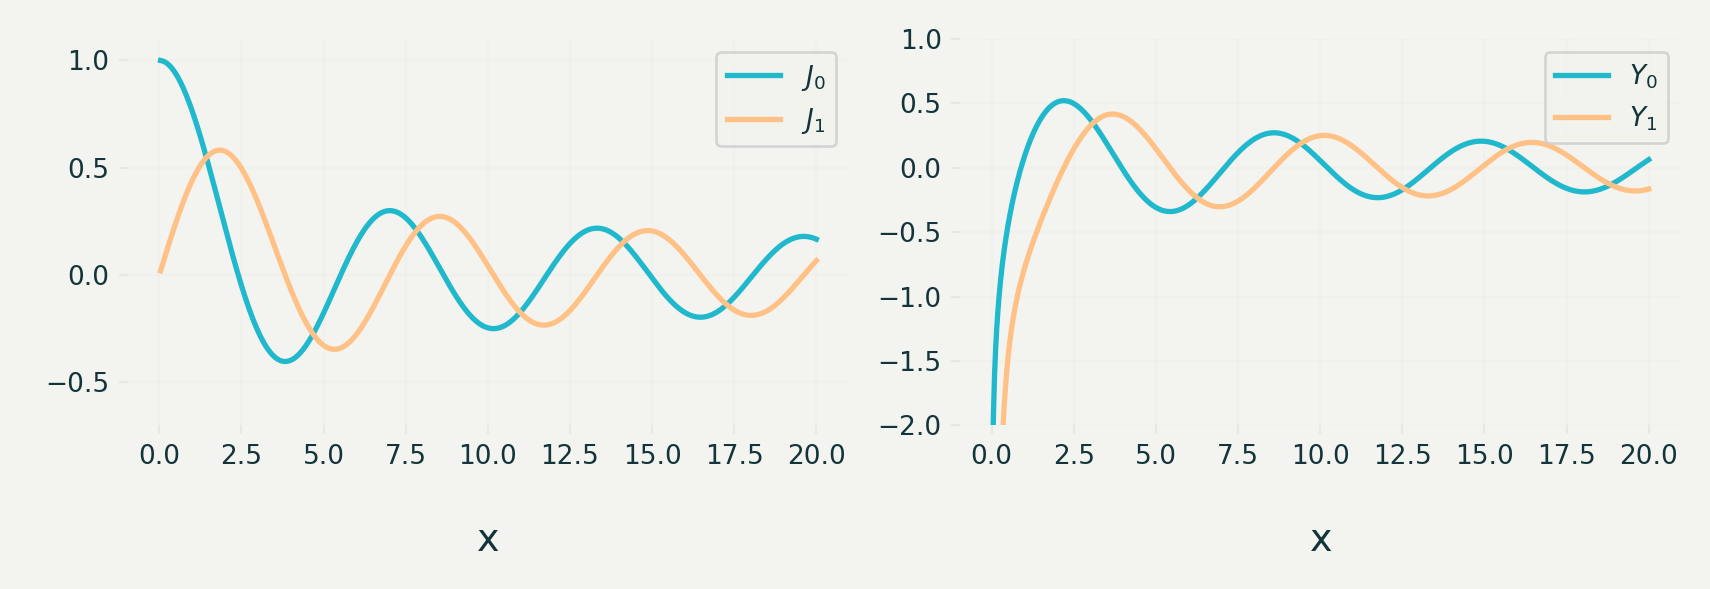
\includegraphics[width=.91\textwidth]{figures/bessel.png}
\caption{Функции Бесселя первого и второго рода порядков $0$ и $1$. Для $Y_\nu$ вертикальный диапазон ограничен: при $x\to0+$ функции неограниченны.}
\end{figure}
\FloatBarrier

\subsection{Стандартные краевые задачи и нормы}
Рассмотрим задачу
\begin{equation}\label{eq:SLB}
-(xy')'+\frac{\nu^2}{x}y=\lambda xy,
\quad 0<x<R,\quad |y(0)|<\infty,\quad \nu\ge0.
\end{equation}
При $\lambda=\kappa^2>0$ ограниченность исключает $Y_\nu$, поэтому $y=J_\nu(\kappa x)$. Обозначим $z=\kappa R$. Условия на правом конце дают
\begin{center}
\begin{tabular}{lll}\toprule
Род & Условие при $x=R$ & Уравнение для $z>0$\\\midrule
I & $y(R)=0$ & $J_\nu(z)=0$\\
II & $y'(R)=0$ & $J_\nu'(z)=0$\\
III & $y'(R)+hy(R)=0$, $h\ge0$ & $zJ_\nu'(z)+hRJ_\nu(z)=0$\\\bottomrule
\end{tabular}
\end{center}
Если $z_k$ --- положительные корни соответствующего уравнения, то
\[
\lambda_k=\frac{z_k^2}{R^2},\qquad X_k(x)=J_\nu(z_kx/R).
\]
Случай $\lambda=0$ проверяется отдельно: ограниченное решение пропорционально $x^\nu$ (при $\nu=0$ --- константе). Поэтому среди перечисленных условий нулевая мода существует только при $\nu=0$ и условии II рода, включая $h=0$ в III роде:
\[
\lambda_0=0,\qquad X_0=1,\qquad \norm{X_0}_x^2=R^2/2.
\]
Корень $z=0$ формальных уравнений нельзя автоматически считать дополнительной собственной функцией.

Скалярное произведение имеет вес $x$:
\[
\ip{f}{g}_x=\int_0^R x f(x)\overline{g(x)}\dd x.
\]
Из уравнения Бесселя непосредственным дифференцированием получается
\[
\frac{\mathrm d}{\mathrm dz}\left\{\frac{z^2}{2}
\left[J_\nu'(z)^2+\left(1-\frac{\nu^2}{z^2}\right)J_\nu(z)^2\right]\right\}=zJ_\nu(z)^2.
\]
После интегрирования и замены переменной:
\begin{equation}\label{eq:normB}
\norm{X_k}_x^2=\frac{R^2}{2}
\left[J_\nu'(z_k)^2+\left(1-\frac{\nu^2}{z_k^2}\right)J_\nu(z_k)^2\right].
\end{equation}
В частности, для I рода $\norm{X_k}_x^2=R^2J_{\nu+1}(z_k)^2/2$. Для II рода --- $R^2(1-\nu^2/z_k^2)J_\nu(z_k)^2/2$. Для III рода --- $R^2[1+((hR)^2-\nu^2)/z_k^2]J_\nu(z_k)^2/2$.

\section{Многочлены Лежандра}
\subsection{Собственные значения, функции и нормы}
Для уравнения Лежандра ставится условие ограниченности на обоих концах:
\begin{equation}\label{eq:Leg}
-((1-x^2)y')'=\lambda y,\qquad -1<x<1,\qquad |y(\pm1)|<\infty.
\end{equation}
Подстановка $y=\sum a_kx^k$ приводит к рекурсии
\[
a_{k+2}=\frac{k(k+1)-\lambda}{(k+1)(k+2)}a_k.
\]
При $\lambda=n(n+1)$ ряд соответствующей чётности обрывается. Ограниченное на обоих концах решение --- многочлен Лежандра. Стандартная нормировка $P_n(1)=1$ задаётся формулой Родрига:
\begin{equation}\label{eq:Rod}
\lambda_n=n(n+1),\quad
P_n(x)=\frac1{2^nn!}\frac{\mathrm d^n}{\mathrm dx^n}(x^2-1)^n,
\qquad n=0,1,\ldots.
\end{equation}
Ортогональность многочленам меньшей степени следует из $n$ интегрирований по частям в \eqref{eq:Rod}: все граничные члены обращаются в нуль. Старший коэффициент равен $(2n)!/[2^n(n!)^2]$, откуда ещё одно применение формулы Родрига даёт
\begin{equation}\label{eq:normL}
\int_{-1}^1 P_nP_k\dd x=0\ (n\ne k),\qquad
\norm{P_n}^2=\int_{-1}^1P_n^2\dd x=\frac2{2n+1}.
\end{equation}
Полнота многочленов в $L^2(-1,1)$ и ортогональность исключают другие собственные значения задачи \eqref{eq:Leg}.

Для присоединённого уравнения фиксируем целое $m\ge0$:
\begin{equation}\label{eq:assoc}
-((1-x^2)y')'+\frac{m^2}{1-x^2}y=\lambda y,
\qquad |y(\pm1)|<\infty.
\end{equation}
Дифференцируя уравнение для $P_n$ $m$ раз и умножая результат на $(1-x^2)^{m/2}$, получаем
\begin{equation}\label{eq:assocsol}
\lambda_n=n(n+1),\qquad
P_n^m(x)=(-1)^m(1-x^2)^{m/2}\frac{\mathrm d^mP_n}{\mathrm dx^m},
\quad n=m,m+1,\ldots.
\end{equation}
Здесь принята фаза Кондона--Шортли $(-1)^m$. При $m>0$ ограниченные собственные функции обращаются в нуль на концах. Второе независимое решение неограниченно.

При фиксированном $m$ собственные функции ортогональны с весом $1$. Их нормы получаются последовательным интегрированием по частям:
\[
\int_{-1}^1(P_n^m)^2\dd x
=(n-m+1)(n+m)\int_{-1}^1(P_n^{m-1})^2\dd x.
\]
С учётом \eqref{eq:normL} имеем
\begin{equation}\label{eq:normA}
\norm{P_n^m}^2=\frac{2(n+m)!}{(2n+1)(n-m)!}.
\end{equation}
При фиксированном $m$ полнота следует также из вида $(1-x^2)^{m/2}q(x)$: ортогональность функции $f\in L^2$ всем таким многочленам означает, что $f(x)(1-x^2)^{m/2}$ ортогональна всем полиномам, а значит равна нулю почти всюду. Поэтому \eqref{eq:assocsol} исчерпывает спектр задачи.

\subsection{Производящая функция и рекуррентные формулы}
Производящая функция имеет вид
\begin{equation}\label{eq:gen}
G(x,t)=\frac1{\sqrt{1-2xt+t^2}}=\sum_{n=0}^{\infty}P_n(x)t^n,
\qquad |t|<1,\quad |x|\le1.
\end{equation}
Действительно, $G(x,0)=1$, а тождество
$(1-2xt+t^2)G_t=(x-t)G$ даёт после сравнения коэффициентов
\begin{equation}\label{eq:recL}
(n+1)P_{n+1}=(2n+1)xP_n-nP_{n-1},\quad
P_0=1,\quad P_1=x.
\end{equation}
Эта рекурсия определяет те же многочлены, что и формула Родрига. Из производных \eqref{eq:gen} также следуют
\[
(1-x^2)P_n'=n(P_{n-1}-xP_n),\qquad
P_{n+1}'-P_{n-1}'=(2n+1)P_n.
\]
Для присоединённых функций дифференцирование \eqref{eq:recL} даёт
\[
(n-m+1)P_{n+1}^m=(2n+1)xP_n^m-(n+m)P_{n-1}^m.
\]
Например,
\[
P_2=\tfrac12(3x^2-1),\quad P_3=\tfrac12(5x^3-3x),\quad
P_4=\tfrac18(35x^4-30x^2+3),\quad
P_5=\tfrac18(63x^5-70x^3+15x).
\]

\begin{figure}[htbp]\centering
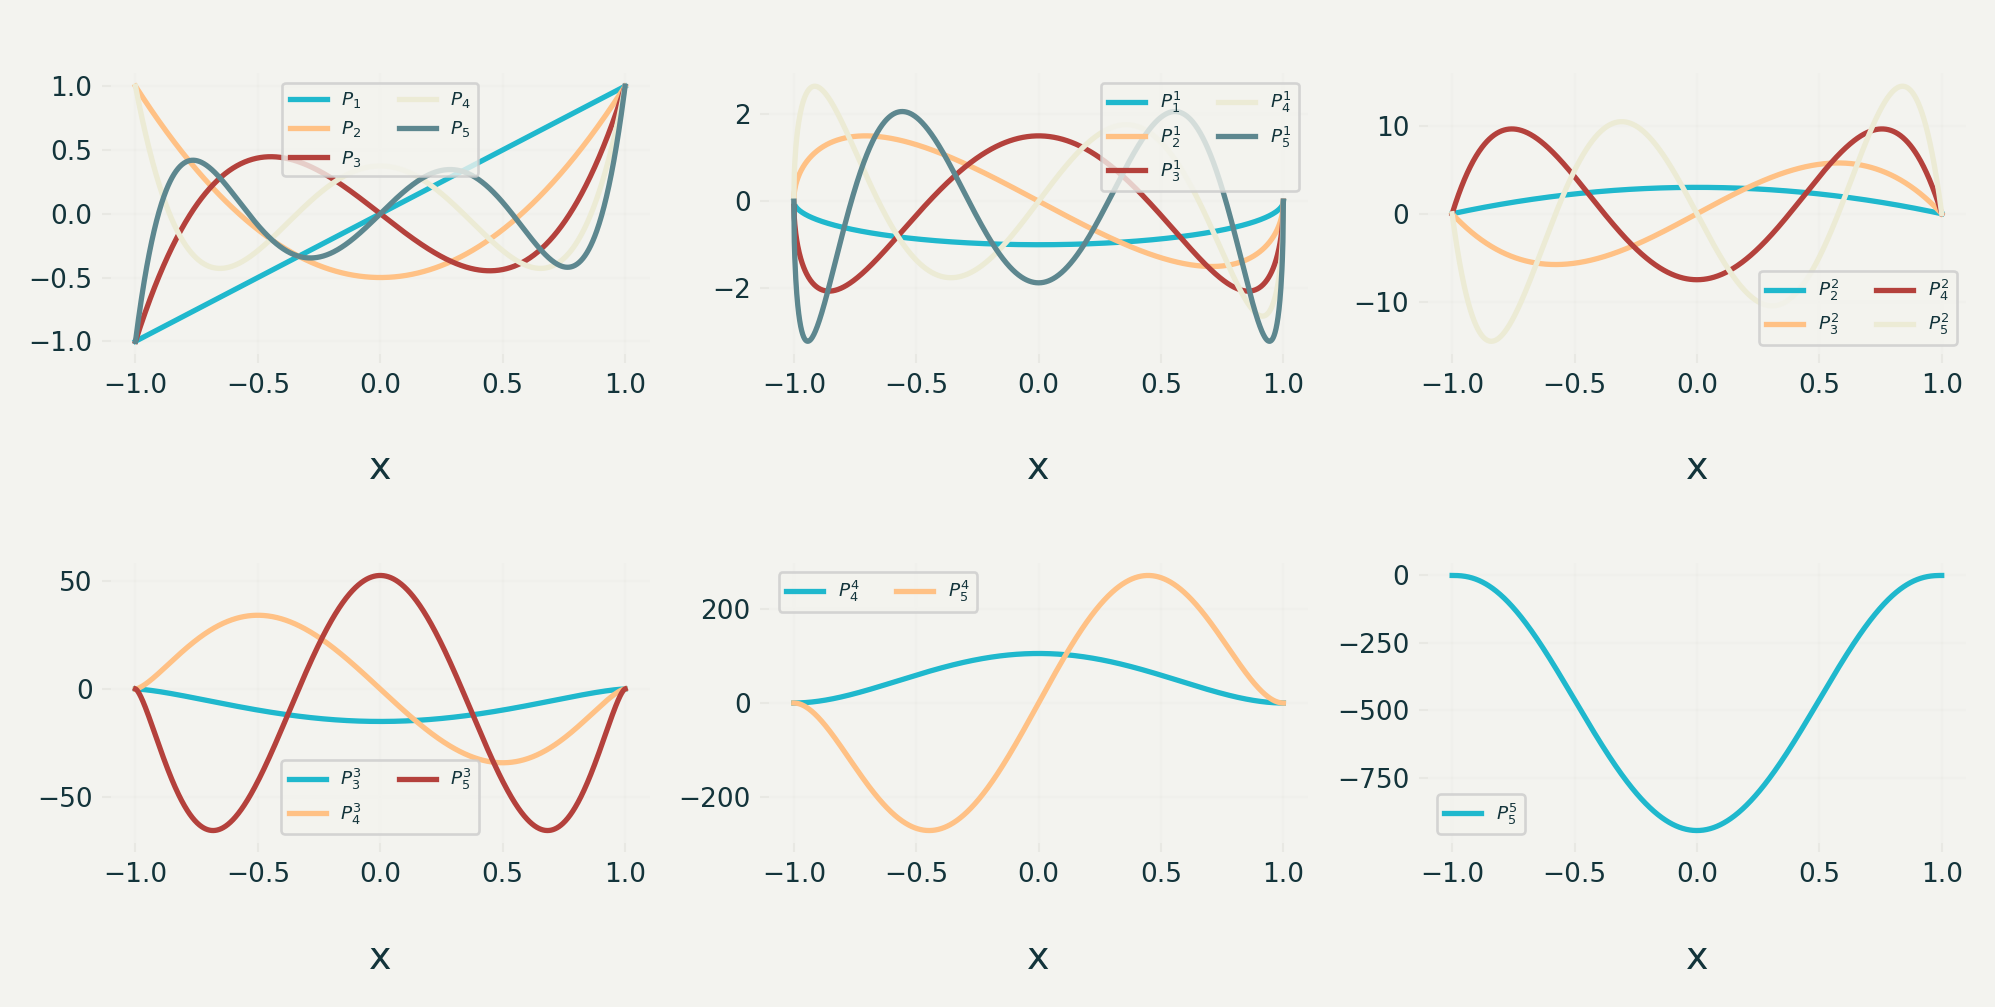
\includegraphics[width=\textwidth]{figures/legendre.png}
\caption{Многочлены $P_n$ и присоединённые функции $P_n^m$ для всех $1\le n\le5$, $0\le m\le n$. При нечётном $m$ функции $P_n^m$ не являются многочленами по $x$.}
\end{figure}

\section{Основные спектральные свойства}
Приведём пять свойств и их обоснование для рассмотренных задач. На вырожденных концах вместо обычного краевого условия требуется ограниченность.

\begin{enumerate}
\item \emph{Собственные значения вещественны и неотрицательны.}
Умножение $-(py')'+qy=\lambda wy$ на $\overline y$ и интегрирование даёт
\begin{equation}\label{eq:energy}
\lambda\int w|y|^2\dd x=
\int(p|y'|^2+q|y|^2)\dd x-[p y'\overline y]_{a}^{b}.
\end{equation}
Для Бесселя $p=w=x$, $q=\nu^2/x$. Правая граница при III роде добавляет $Rh|y(R)|^2\ge0$. Для Лежандра $p=1-x^2$, $w=1$, $q=0$ или $m^2/(1-x^2)$. На вырожденных концах граничные члены равны нулю по поведению ограниченных решений. Правая часть вещественна и неотрицательна. Равенство нулю возможно только для постоянной функции при $q=0$ и допускающих её условиях: $\nu=0$ и II род у Бесселя, $n=0$ у Лежандра.

\item \emph{Собственные значения простые. Функция определяется с точностью до множителя.}
В задаче Бесселя правое краевое условие задаёт одну линейную связь между $X(R)$ и $X'(R)$. Поэтому начальные данные двух собственных функций при одном $\lambda$ пропорциональны. По единственности решения задачи Коши сами функции также пропорциональны. Для уравнения Лежандра и присоединённого уравнения ограниченность при $x=-1$ оставляет только одно независимое решение, поскольку второе неограниченно. Правое условие отбирает допустимые значения $\lambda$, не увеличивая число независимых решений.

\item \emph{Спектр счётен, неограничен сверху и не имеет конечных точек накопления.}
Для Бесселя из \eqref{eq:asymp} следуют бесконечные последовательности положительных корней краевых уравнений. Они изолированы по аналитичности, причём $z_k=\pi k+O(1)$ при фиксированном порядке и роде условия. Для Лежандра спектр явно равен $n(n+1)$, где $n\ge0$ или $n\ge m$ соответственно. Других собственных значений нет в силу полноты, указанной ниже.

\item \emph{Собственные функции различных собственных значений ортогональны.}
Умножим уравнение для $X_n$ на $\overline{X_k}$, а сопряжённое уравнение для $X_k$ на $X_n$. После вычитания и интегрирования по частям граничные члены обращаются в нуль в силу краевых условий. Получаем
\[
(\lambda_n-\lambda_k)\int_a^b wX_n\overline{X_k}\dd x=0.
\]
Поэтому при $\lambda_n\ne\lambda_k$ интеграл равен нулю. Нормы вычислены в \eqref{eq:normB}, \eqref{eq:normL}, \eqref{eq:normA}. Деление на норму даёт ортонормированную систему.

\item \emph{Система собственных функций полна в соответствующем весовом пространстве.}
Для $P_n$ и $P_n^m$ это доказано выше через плотность многочленов. Для Бесселя ограниченное решение на левом конце и выбранное условие на правом задают самосопряжённую задачу с компактным обратным оператором после положительного сдвига спектра. Краткое обоснование компактности: ядро Грина квадратично интегрируемо с мерой $x\dd x\,s\dd s$. При нуле его возможная логарифмическая особенность интегрируема, а при $\nu>0$ возникают ограниченные отношения $(\min(x,s)/\max(x,s))^\nu$. Спектральная теорема для компактного самосопряжённого оператора даёт полноту. Например, для I рода при $\nu=0$ ядро обратного оператора равно $\ln(R/\max(x,s))$. При нулевой моде используется сдвиг $A+I$, не меняющий собственных функций.
\end{enumerate}
Дополнительно, нули положительных мод просты: равенства $X(x_0)=X'(x_0)=0$ во внутренней точке по теореме единственности дали бы $X\equiv0$. У $P_n$ ровно $n$ внутренних нулей, у $P_n^m$ --- $n-m$, у $k$-й функции Бесселя для I рода --- $k-1$.

\section{Разложения и сходимость}
Для I рода положим $j_{\nu,k}=z_k$, $J_\nu(j_{\nu,k})=0$. Формальный ряд Фурье--Бесселя и его коэффициенты:
\begin{equation}\label{eq:FB}
f(x)\sim\sum_{k=1}^{\infty}a_kJ_\nu(j_{\nu,k}x/R),\qquad
a_k=\frac{2\int_0^R xf(x)J_\nu(j_{\nu,k}x/R)\dd x}
{R^2J_{\nu+1}(j_{\nu,k})^2}.
\end{equation}
Для II и III рода берутся соответствующие корни и нормы \eqref{eq:normB}. При наличии нулевой моды она добавляется отдельно.

Ряд Фурье--Лежандра имеет вид
\begin{equation}\label{eq:FL}
f(x)\sim\sum_{n=0}^{\infty}b_nP_n(x),\qquad
b_n=\frac{2n+1}{2}\int_{-1}^1 f(x)P_n(x)\dd x.
\end{equation}
Для фиксированного $m$ аналогично
\[
f(x)\sim\sum_{n=m}^{\infty}b_n^{(m)}P_n^m(x),\qquad
b_n^{(m)}=\frac{(2n+1)(n-m)!}{2(n+m)!}
\int_{-1}^1f(x)P_n^m(x)\dd x.
\]
Полнота обеспечивает сходимость \eqref{eq:FB} в $L^2((0,R),x\dd x)$ и \eqref{eq:FL} в $L^2(-1,1)$ для любой функции из соответствующего пространства. Для ортонормированных функций $\phi_k$ выполняются
\begin{equation}\label{eq:parseval}
\norm{f-S_N}^2=\norm f^2-\sum_{k=0}^{N-1}|\ip f{\phi_k}|^2\longrightarrow0.
\end{equation}
Кроме того, $S_N$ --- наилучшее среднеквадратичное приближение в линейной оболочке первых $N$ функций: для любой $v$ из этой оболочки
$\norm{f-v}^2=\norm{f-S_N}^2+\norm{S_N-v}^2$.

Если функция кусочно гладкая на замкнутом отрезке, внутри интервала соответствующий ряд сходится к $f$ в точках непрерывности и к полусумме односторонних пределов в точках скачка. Сходимость в среднем сама по себе не означает равномерную сходимость. В частности, ряд Бесселя I рода равен нулю при $x=R$. При $f(R)\ne0$ он не может сходиться к $f$ равномерно на всём отрезке. Достаточное условие равномерной сходимости --- достаточно гладкая функция с согласованными краевыми условиями. Для Лежандра, например, достаточно $f\in C^2[-1,1]$. Утверждения о внутренних точках не заменяют отдельной проверки вырожденных концов.

Сравним частичные суммы по $N=10$ функциям для
\[
f_1(t)=e^t,\qquad f_2(t)=|t-0.4|,\qquad f_3(t)=(1-t)e^{-8t},\quad 0\le t\le1.
\]
Для сопоставления в одной норме $L^2(0,1)$ используем ортонормированные системы
\begin{align*}
\phi_k^{\mathrm B}(t)&=\frac{J_0(j_{0,k+1}\sqrt t)}{|J_1(j_{0,k+1})|},\\
\phi_k^{\mathrm L}(t)&=\sqrt{2k+1}\,P_k(2t-1),\\
\phi_0^{\mathrm C}(t)&=1,\qquad \phi_k^{\mathrm C}(t)=\sqrt2\cos(k\pi t),\quad k\ge1.
\end{align*}
В первых двух строках $k\ge0$. Замена $t=r^2$ в бесселевой системе приводит вес к единице. Частичная сумма и квадрат ошибки имеют вид
\[
S_{10}(t)=\sum_{k=0}^9\ip f{\phi_k}\phi_k(t),\qquad E_{10}^2=\int_0^1|f(t)-S_{10}(t)|^2\dd t.
\]
\begin{figure}[htbp]\centering
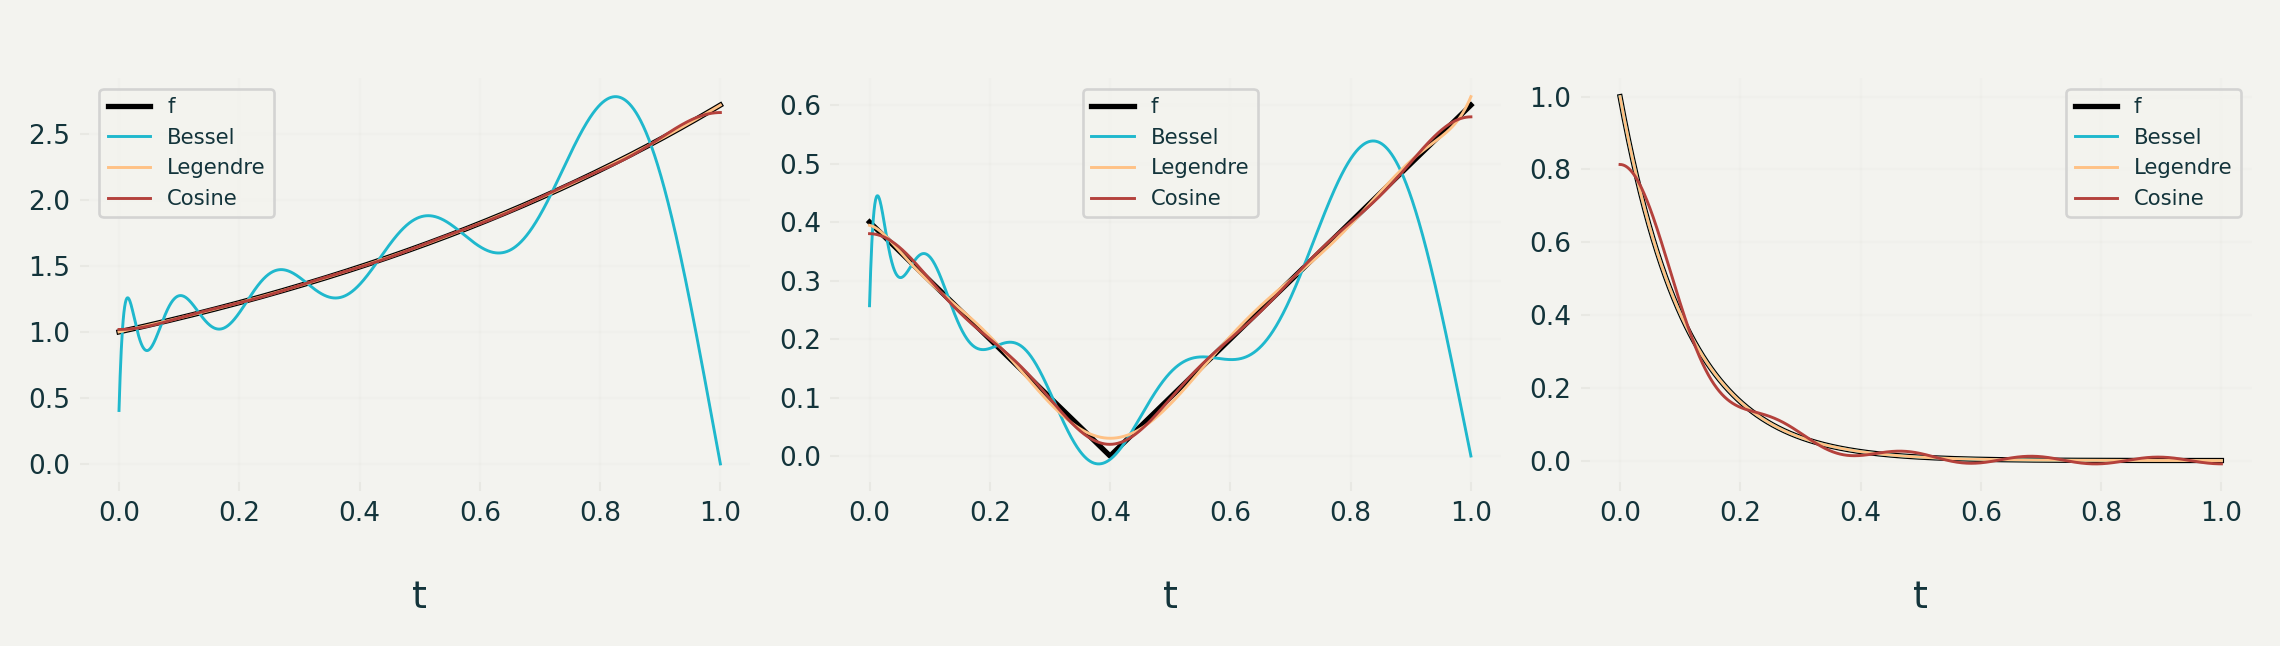
\includegraphics[width=\textwidth]{figures/approximations.png}
\caption{Приближения выбранных функций по десяти функциям бесселевой, лежандровой и косинусной систем.}
\end{figure}
\begin{figure}[htbp]\centering
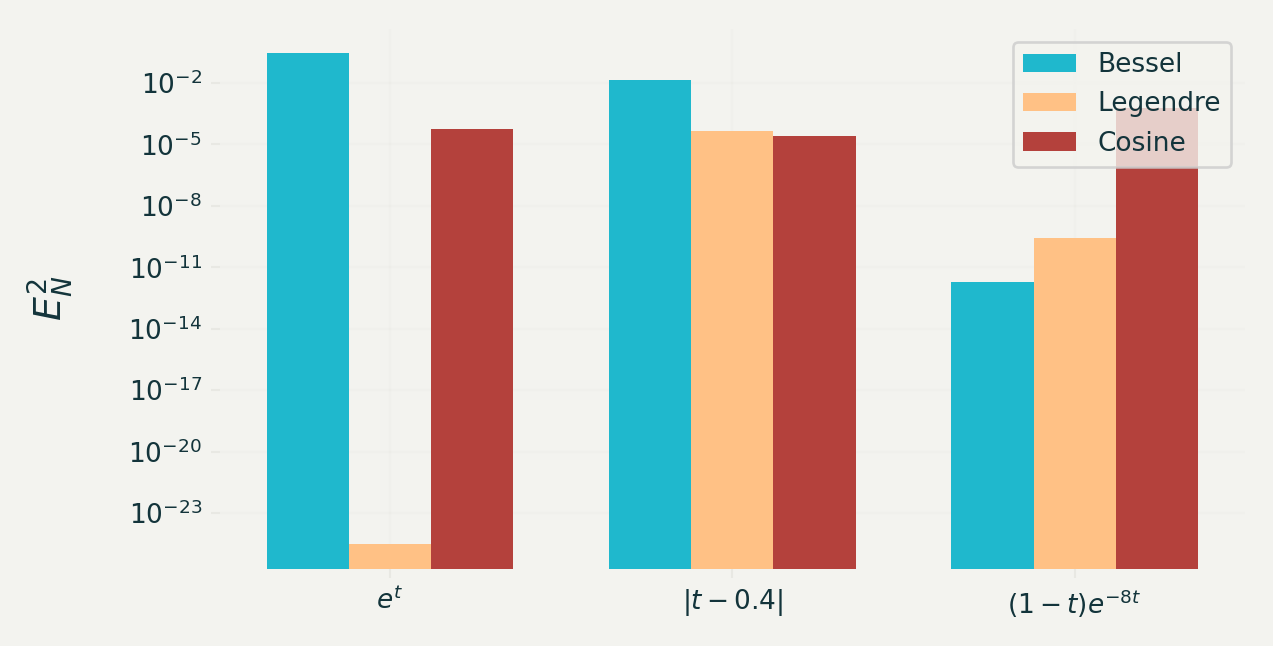
\includegraphics[width=.70\textwidth]{figures/errors.png}
\caption{Квадраты ошибок $E_{10}^2$ в общей норме $L^2(0,1)$.}
\end{figure}
\FloatBarrier
Для $e^t$ наилучшее приближение даёт система Лежандра, хорошо передающая гладкую функцию полиномами. Для $|t-0.4|$ при выбранном числе членов немного точнее косинусная система, а излом замедляет сходимость. Для $(1-t)e^{-8t}$ лучше бесселева система, согласованная со значением $f(1)=0$. Несогласованность значения на правом конце ухудшает бесселево приближение первых двух функций. Эти сравнения относятся к выбранным функциям и числу членов.

\section{Физические задачи}
\subsection{Свободные колебания тяжёлой нити}
Пусть $x$ отсчитывается от свободного нижнего конца, $0\le x\le L$, $\rho$ --- постоянная линейная плотность. Натяжение равно весу нижележащего участка: $T(x)=\rho gx$. Баланс поперечных сил $\rho u_{tt}=(Tu_x)_x$ приводит к задаче
\begin{equation}\label{eq:string1}
u_{tt}=g(xu_x)_x,\quad u(L,t)=0,\quad |u(0,t)|<\infty,
\quad u(x,0)=\varphi(x),\quad u_t(x,0)=\psi(x).
\end{equation}
У свободного конца естественное условие $\lim_{x\to0+}xu_x=0$ следует из регулярности решения. Ищем $u=X(x)T(t)$:
\[
(xX')'+\frac{\omega^2}{g}X=0,\qquad T''+\omega^2T=0.
\]
Замена $z=2\omega\sqrt{x/g}$ даёт уравнение Бесселя нулевого порядка. Ограниченность оставляет $J_0$, а закрепление сверху даёт
\[
\omega_k=\frac{j_{0,k}}2\sqrt{\frac gL},\qquad
X_k(x)=J_0(j_{0,k}\sqrt{x/L}),\qquad k=1,2,\ldots.
\]
Подстановкой $r=\sqrt{x/L}$ в интеграл нормы получаем
\[
\norm{X_k}^2=\int_0^L X_k^2\dd x=LJ_1(j_{0,k})^2.
\]
Искомое решение:
\begin{equation}\label{eq:sol1}
u(x,t)=\sum_{k=1}^{\infty}
\left(A_k\cos\omega_kt+\frac{C_k}{\omega_k}\sin\omega_kt\right)X_k(x),
\end{equation}
\[
A_k=\frac{\int_0^L\varphi(x)X_k(x)\dd x}{LJ_1(j_{0,k})^2},\qquad
C_k=\frac{\int_0^L\psi(x)X_k(x)\dd x}{LJ_1(j_{0,k})^2}.
\]
Начальные функции предполагаются согласованными с закреплением при $x=L$. При достаточной гладкости ряд задаёт классическое решение, а для данных из соответствующего энергетического пространства --- обобщённое.

\subsection{Малые колебания вращающейся струны}
Термин «невесомая» в условии понимается как пренебрежение действием силы тяжести, но не инерцией: линейная плотность $\rho>0$. Иначе распределённое центробежное натяжение не возникает. Пусть $x$ --- расстояние от оси, $0\le x\le L$, $\Omega>0$ --- угловая скорость. Натяжение обеспечивает центростремительное ускорение части струны $[x,L]$:
\[
T(x)=\int_x^L\rho\Omega^2s\dd s
=\frac{\rho\Omega^2}{2}(L^2-x^2).
\]
Для малых смещений по нормали к плоскости вращения:
\begin{equation}\label{eq:string2}
u_{tt}=\frac{\Omega^2}{2}\bigl((L^2-x^2)u_x\bigr)_x,
\quad u(0,t)=0,\quad |u(L,t)|<\infty,
\end{equation}
\[
u(x,0)=\varphi(x),\qquad u_t(x,0)=\psi(x).
\]
На свободном конце $T(L)=0$. Условие регулярности даёт $\lim_{x\to L-}(L^2-x^2)u_x=0$. При $\xi=x/L$ разделение переменных приводит к
\[
((1-\xi^2)X')'+\lambda X=0,\quad X(0)=0,\quad |X(1)|<\infty,
\qquad \lambda=\frac{2\omega^2}{\Omega^2}.
\]
Нечётное продолжение на $[-1,1]$ сводит задачу к задаче Лежандра. Условие $P_n(0)=0$ оставляет только нечётные степени:
\[
X_k(x)=P_{2k+1}(x/L),\qquad
\omega_k=\Omega\sqrt{\frac{(2k+1)(2k+2)}2},\quad k=0,1,\ldots.
\]
По чётности произведения и формуле \eqref{eq:normL}
\[
\int_0^L X_k^2\dd x=\frac{L}{4k+3}.
\]
Решение выражается рядом
\begin{equation}\label{eq:sol2}
u(x,t)=\sum_{k=0}^{\infty}
\left(A_k\cos\omega_kt+\frac{C_k}{\omega_k}\sin\omega_kt\right)
P_{2k+1}(x/L),
\end{equation}
\[
A_k=\frac{4k+3}{L}\int_0^L\varphi(x)P_{2k+1}(x/L)\dd x,\qquad
C_k=\frac{4k+3}{L}\int_0^L\psi(x)P_{2k+1}(x/L)\dd x.
\]
В частности, $\omega_0=\Omega$. Длина сокращается из частот, поскольку центробежное натяжение само пропорционально $L^2$. Как и в первой задаче, начальные данные должны быть согласованы с закреплением, а классическая разрешимость требует достаточной гладкости.

\end{document}
